\section{Generalisierung}
\label{sec:Kap-8.5}

Aus Abschnitt~4.3 wissen Sie, dass in Generalisierungsbeziehungen die Oberklassen Eigenschaften an ihre Unterklasse(n) vererben. Die Unterklassen wiederum können Eigenschaften zu dem Ererbten hinzufügen oder auch Ererbtes verändern, um ihre Spezialisierung zu charakterisieren. Neben den Eigenschaften, die durch Attribute der Klassen abgebildet sind, gilt dieses Vererbungsprinzip auch für die Opera\-tionen der Oberklassen. Abbildung~\ref{fig:generalisierung_baeume} zeigt anknüpfend an das Baumbeispiel aus Abschnitt~4.3 wieder eine Generalisierungsbeziehung aus dem Baumkontext.

\vspace{\baselineskip} %%% für Druck

\begin{figure}[h!]
	\centering
	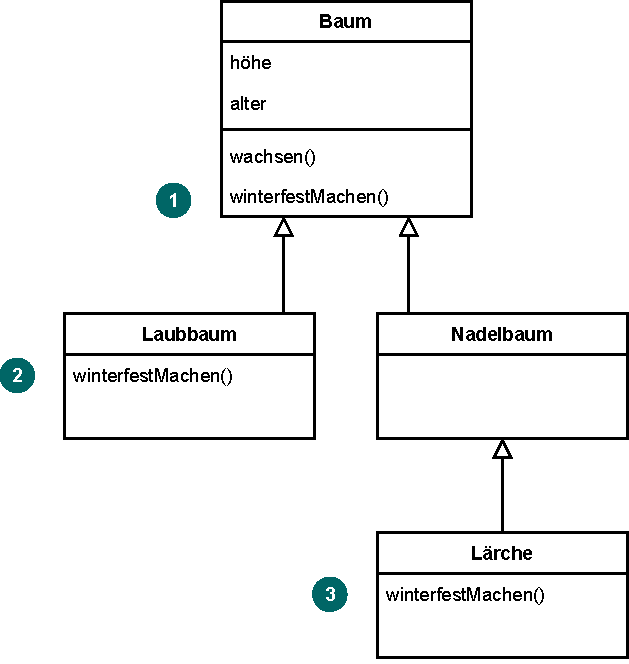
\includegraphics[scale=1.0]{Bilder/Kapitel-8/generalisierung_baeume.pdf}
	\caption{Vererbung von Operationen}
	\label{fig:generalisierung_baeume}
\end{figure}

\vspace{\baselineskip} %%% für Druck

\textbf{Konzeptuell} ist eine Lärche in diesem Beispiel sowohl eine Lärche, als auch ein Nadelbaum, als auch ein Baum. \textbf{Implementierungstechnisch} gesehen gehört ein Objekt nur zu genau einer Klasse. Ein Lärche-Objekt wird als Instanz der Klasse \sttpUMLText{Lärche} erzeugt. Die Lärche-Instanz besitzt aber auch Attribute und Operationen, die die Klassen \sttpUMLText{Nadelbaum} und \sttpUMLText{Baum} definiert haben. In der UML-Darstellung werden die vererbten Attribute und Operationen nur in der Oberklasse notiert, in der sie definiert werden. In den Unterklassen, die diese Attribute und Operationen erben, werden sie nur dann aufgeführt, wenn die Unterklasse sie verändert (programmiertechnisch gesprochen: überschreibt). 

Für die dargestellten Klassen sind einige Attribute und Operationen angegeben. Die Attribute \sttpUMLText{höhe} und \sttpUMLText{alter} sowie die Operation \sttpUMLText{wachsen()} der Klasse Baum werden auf alle Unterklassen in der Generalisierungshierarchie vererbt. Insofern besitzen sowohl die Klassen \sttpUMLText{Laubbaum} und \sttpUMLText{Nadelbaum} als auch die in dritter Generalisierungsebene angesiedelte Klasse \sttpUMLText{Lärche} die beiden Attribute und die Operation \sttpUMLText{wachsen()}. 

\vspace{1mm} %%% für Druck

An drei Stellen im Diagramm finden wir die Operation \sttpUMLText{winterfestMachen()}. In der Klasse \sttpUMLText{Baum} (Nr. 1) umfasst sie alle Aktionen, die alle Arten von Bäumen vor dem Winter ausführen, sagen wir, das wäre die Verengung der Wasserleitbahnen im Stamm und die Herabsetzung des Gefrierpunkts des Zellsafts durch Einlagern von Zuckern und Eiweißen. In der Klasse \sttpUMLText{Laubbaum} (Nr. 2) kann die Operation \sttpUMLText{winterfestMachen()} der Oberklasse \sttpUMLText{Baum} überschrieben werden, \zb weil ein Laubbaum vor dem Winter zusätzlich noch seine Blätter abwerfen soll. In der Klasse \sttpUMLText{Nadelbaum} überschreiben wir die Operation dagegen nicht, da die Operation der Oberklasse \sttpUMLText{Baum} das Verhalten von Nadelbäumen schon adäquat abdeckt. Der Aufruf der Operation \sttpUMLText{winterfestMachen()} auf einer Nadelbaum-Instanz würde dazu führen, dass die geerbte Operation der Oberklasse \sttpUMLText{Baum} ausgeführt wird. In der Klasse \sttpUMLText{Lärche} (Nr. 3) überschreiben wir die Operation der Oberklasse \sttpUMLText{Baum}, denn die Lärche ist eine von zwei Nadelbaum-Arten, die ihre Nadeln abwirft, daher reicht die Implementierung der Operation in der Klasse \sttpUMLText{Baum} für die Lärche im Gegensatz zu anderen Nadelbaum-Objekten nicht aus. 

\vspace{1mm} %%% für Druck

In der objektorientierten Programmierung kann eine Instanz einer Unterklasse in der Rolle einer Instanz der Oberklasse agieren. \marginline{Polymorphie} So kann zum Beispiel eine Lärchen-Instanz auch die Rolle eines Nadelbaums oder die Rolle eines Baums annehmen. In einem solchen Fall zeigt sie nur das Verhalten der entsprechenden Oberklasse und nicht dasjenige ihrer eigenen spezialisierten Klasse. Das bedeutet, wenn die Lärchen-Instanz als Lärche agiert, führt sie ihre eigene winterfestMachen()-Operation aus. Agiert sie dagegen als Nadelbaum oder als Baum führt sie die entsprechende Operation der Klasse \sttpUMLText{Baum} aus. Das Agieren-können einer Unterklassen-Instanz als Instanz einer Oberklasse bezeichnet man in der Objektorientierung als Polymorphie. 

\vspace{1mm} %%% für Druck

Es gibt einen konzeptionellen Unterschied zwischen Generalisierung und Vererbung: Generalisierung ist ein semantisches Konzept. \marginline{Generalisierung vs. Vererbung} Es geht darum, Realwelt-Hierarchien im Modell abbilden zu können. Es beinhaltet nicht, „irgendwelche“ Gemeinsamkeiten in einer Klasse zusammenzufassen. Nur weil ein Stuhl, ein Tisch und ein Hund alle vier Beine haben, sind sie keine Spezialisierungen einer Klasse Vierbeiner. In der objektorientierten Programmierung wird vom inhaltlichen Generalisierungsprinzip allerdings häufig abgewichen, indem Oberklassen-Unterklassen-Beziehungen konstruiert werden, weil Implementierungen von Operationen einer Klasse auch in anderen Klassen sinnvoll verwendet werden können. Um solche Oberklassen-Unterklassen-Beziehungen von der Realwelt-orientierten Generalisierung zu unterscheiden, spricht man in objektorientierten Programmiersprachen statt von Generalisierung von Vererbung -- übrigens teilweise auch an den Stellen, an denen es sich wirklich um die Umsetzung einer Generalisierungsbeziehung handelt. Für Klassen, deren (zukünftige) Instanzen von Objekten der Realwelt abgeleitet sind, sollte man im Programm\-code stets versuchen, die natürlichen Generalisierungs\-beziehungen beizubehalten. Zum Beispiel sollten wir die Klasse \sttpUMLText{Lärche} nicht als Spezialisierung der Klasse \sttpUMLText{Laubbaum} entwerfen, auch wenn wir für die Klasse \sttpUMLText{Lärche} genau die winterfestMachen()-Operation der Klasse \sttpUMLText{Laubbaum} gebrauchen könnten.

Vererbung ist ein sehr mächtiges Konzept. Durch geeignet strukturierte Vererbungsbeziehungen kann man Codeduplizierungen vermeiden, aber auch Erweiterungen der Funktionalität vereinfachen, indem man zu einer schon vorhandenen Klasse (ohne diese ändern zu müssen) eine zusätzliche Unterklasse mit der neuen Funktionalität hinzufügt. Wenn zusätzlich sogenannte abstrakte Klassen in den Vererbungs\-hierachien eingesetzt werden, wird das ganze Konzept noch mächtiger.

Eine \textit{abstrakte Klasse} 
\marginline{abstrakte Klasse}
ist eine Klasse, die bewusst nur unvollständig modelliert wird. Unvollständig bedeutet, dass sie Operationen besitzt (sogenannte abstrakte Operationen), die nur aus der Signatur bestehen, aber deren Operationsrumpf nicht ausprogrammiert ist. Konzeptuell ist eine Klasse dann eine abstrakte Klasse, wenn sie mindestens eine solche abstrakte Operation enthält. Ihre anderen Operationen dürften durchaus komplett sein -- die objektorientierten Programmiersprachen sind hier oft strikter, so dass alle Operationen abstrakt sein müssen. In der UML werden abstrakte Klassen über den Zusatz \sttpUMLText{\{abstract\}} gekennzeichnet. Häufiger findet man aber eine zweite, auch zulässige Darstellungsform mit Kursivsetzung von Klassenname und Operationen, wie in Abbildung~\ref{fig:abstrakte_klasse}. 

\vspace{\baselineskip} %%% für Druck

\begin{figure}[h!]
	\centering
	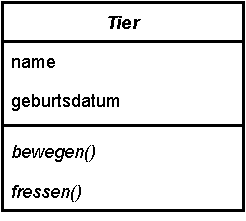
\includegraphics[scale=1.0]{Bilder/Kapitel-8/Abstrakt2.pdf}
	\caption{Eine Klasse \sttpUMLText{Tier} als abstrakte Klasse}
	\label{fig:abstrakte_klasse}
\end{figure}

\vspace{\baselineskip} %%% für Druck

Da abstrakte Klassen abstrakte Operationen haben, kann man keine Instanzen von ihnen bilden. Gebildete Instanzen würden unvollständiges Verhalten auf\-weisen. \mbox{Abstrakte} Klassen werden verwendet, um ihren (nicht-abstrakten) Unter\-klassen Strukturen vorzugeben, nämlich welche Attribute und welche Operationen diese implementieren müssen. Auf diese Weise ist gewährleistet, dass alle Unterklassen entsprechendes Verhalten aufweisen werden, aber in der konkreten Ausgestaltung angepasst an die jeweilige Unterklasse. In Abbildung~\ref{fig:abstrakte_klasse} hat die abstrakte Klasse \sttpUMLText{Tier} die beiden abstrakten Operationen \sttpUMLText{bewegen()} und \sttpUMLText{fressen()}. Diese müssen in den Unterklassen -- sagen wir, das wären die Klassen \sttpUMLText{Elefant} und \sttpUMLText{Meerschweinchen} -- für die jeweilige Klasse geeignet implementiert werden. 